\documentclass[a4paper,twoside,11pt]{article}
\usepackage{a4wide,graphicx,fancyhdr,amsmath,amssymb,amsthm,ifthen,path}
\usepackage[ruled, noline, algo2e, noend]{algorithm2e}
\usepackage{hyperref}
\usepackage{url}
\usepackage{color}
\usepackage{todonotes}
\usepackage{parskip}
\usepackage{subcaption}
\usepackage{etoolbox, array, dcolumn}
\urlstyle{rm}

\setlength\headheight{20pt}
\addtolength\topmargin{-10pt}
\addtolength\footskip{20pt}

\fancypagestyle{plain}{%
	\fancyhf{}
	\fancyfoot[LO,RE]{\sffamily\bfseries 2IV35~--~Visualization}
	\fancyfoot[RO,LE]{\sffamily\bfseries\thepage}
	\renewcommand{\headrulewidth}{0pt}
	\renewcommand{\footrulewidth}{0pt}
}

\pagestyle{fancy}{
\fancyhf{}
\fancyhead[LE]{\sffamily\bfseries Joris Reijrink and Chris Hoedemakers}
\fancyhead[RO]{\sffamily\bfseries Interactive Visualization}
\fancyfoot[LO,RE]{\sffamily\bfseries 2IV35~--~Visualization}
\fancyfoot[RO,LE]{\sffamily\bfseries\thepage}
\renewcommand{\headrulewidth}{1pt}
\renewcommand{\footrulewidth}{0pt}
}

\title{\sffamily\bfseries
\fontsize{22pt}{1pt} Assignment 3 \\[1ex]
\large Interactive Visualization \bigskip}

\author{
	Joris Reijrink \\
	Student number: 0847198 \\
	\texttt{j.reijrink@student.tue.nl}
	\and
	Chris Hoedemakers \\
	Student number: 0661115 \\
	\texttt{c.g.j.j.hoedemakers@student.tue.nl}
}

\date{\today}

\newcounter{cs}

\newcommand{\code}[1]{
	\refstepcounter{cs}
	\begin{center}
	\hspace*{-2.2cm}
	\begin{minipage}{1.103\textwidth}
		\begin{minipage}{0.1\textwidth}%
			\raggedleft
			\footnotesize{\texttt{CS \thecs}}\hspace*{0.3cm}
		\end{minipage}
		\begin{minipage}{0.88\textwidth}%
			\colorbox{gray!20}{
				\begin{minipage}{\textwidth}%
				\fontsize{8pt}{8pt}\texttt{#1}
				\end{minipage}
			}
		\end{minipage}
	\end{minipage}
	\end{center}
	\vspace*{0.3cm}
}
\newcommand{\tab}{\hspace*{0.6cm}}

\newcolumntype{d}[1]{D{.}{.}{#1}}


\begin{document}

\maketitle
\setcounter{page}{1}

\setlength{\parindent}{0cm}
\setlength{\parskip}{0.3cm}

\section{Introduction}\label{sec:intro}
In this project we are given some basic volume visualization application and will implement several additional features in order to enhance this application. To be able to clearly explain the added functionality, we start by shortly describing the initial functioning of the application. 

Technically speaking, it could be argued whether the initial application is even a real raycaster, as it simply takes a slice through the data, and projects this data onto the viewing window (see figure \ref{fig:raycaster0}). The slice is defined in such a way that it always goes exactly through the center of the volume bounding box, and is oriented perpendicular to the view vector \texttt{viewVec}. As the view vector is again perpendicular to the view window, the slice is always parallel to the view window. The width and height of the slice are both defined by the diagonal of the bounding box. This is an obvious choice, because this is the smallest dimension that ensures that no data can ever lie outside of the slice area. 

When looking at the code of the initial application, we observe that all of the above functionality is realized by a function called \texttt{slicer()}, which uses a simple nested for-loop to walk along all the pixels of the view window in horizontal and vertical direction. For each pixel, the value is then determined as follows. First we cast a ray from that pixel, parallel to the view vector. We then determine the $x$-, $y$- and $z$-coordinate of the intersection of this ray with the slice plane. This is done using two additional vectors \texttt{uVec} and \texttt{vVec} that are defined by ...\todo{!}. Once the coordinates are determined, they are passed on to a function called \texttt{getVoxel()}. This function then rounds the three coordinate values in order to obtain the voxel that is closest to the received coordinate (i.e. the nearest neighbor voxel). The value of this voxel is then returned to the slicer function, and passed on to the function \texttt{tFunc.getColor()}, obtains the correct color for the voxel value that was returned by \texttt{getVoxel()}. This color is finally converted into an ARGB color and drawn onto the view window.

\begin{figure}[h!]
    \centering
    \captionsetup{justification=centering,margin=0.5cm}
    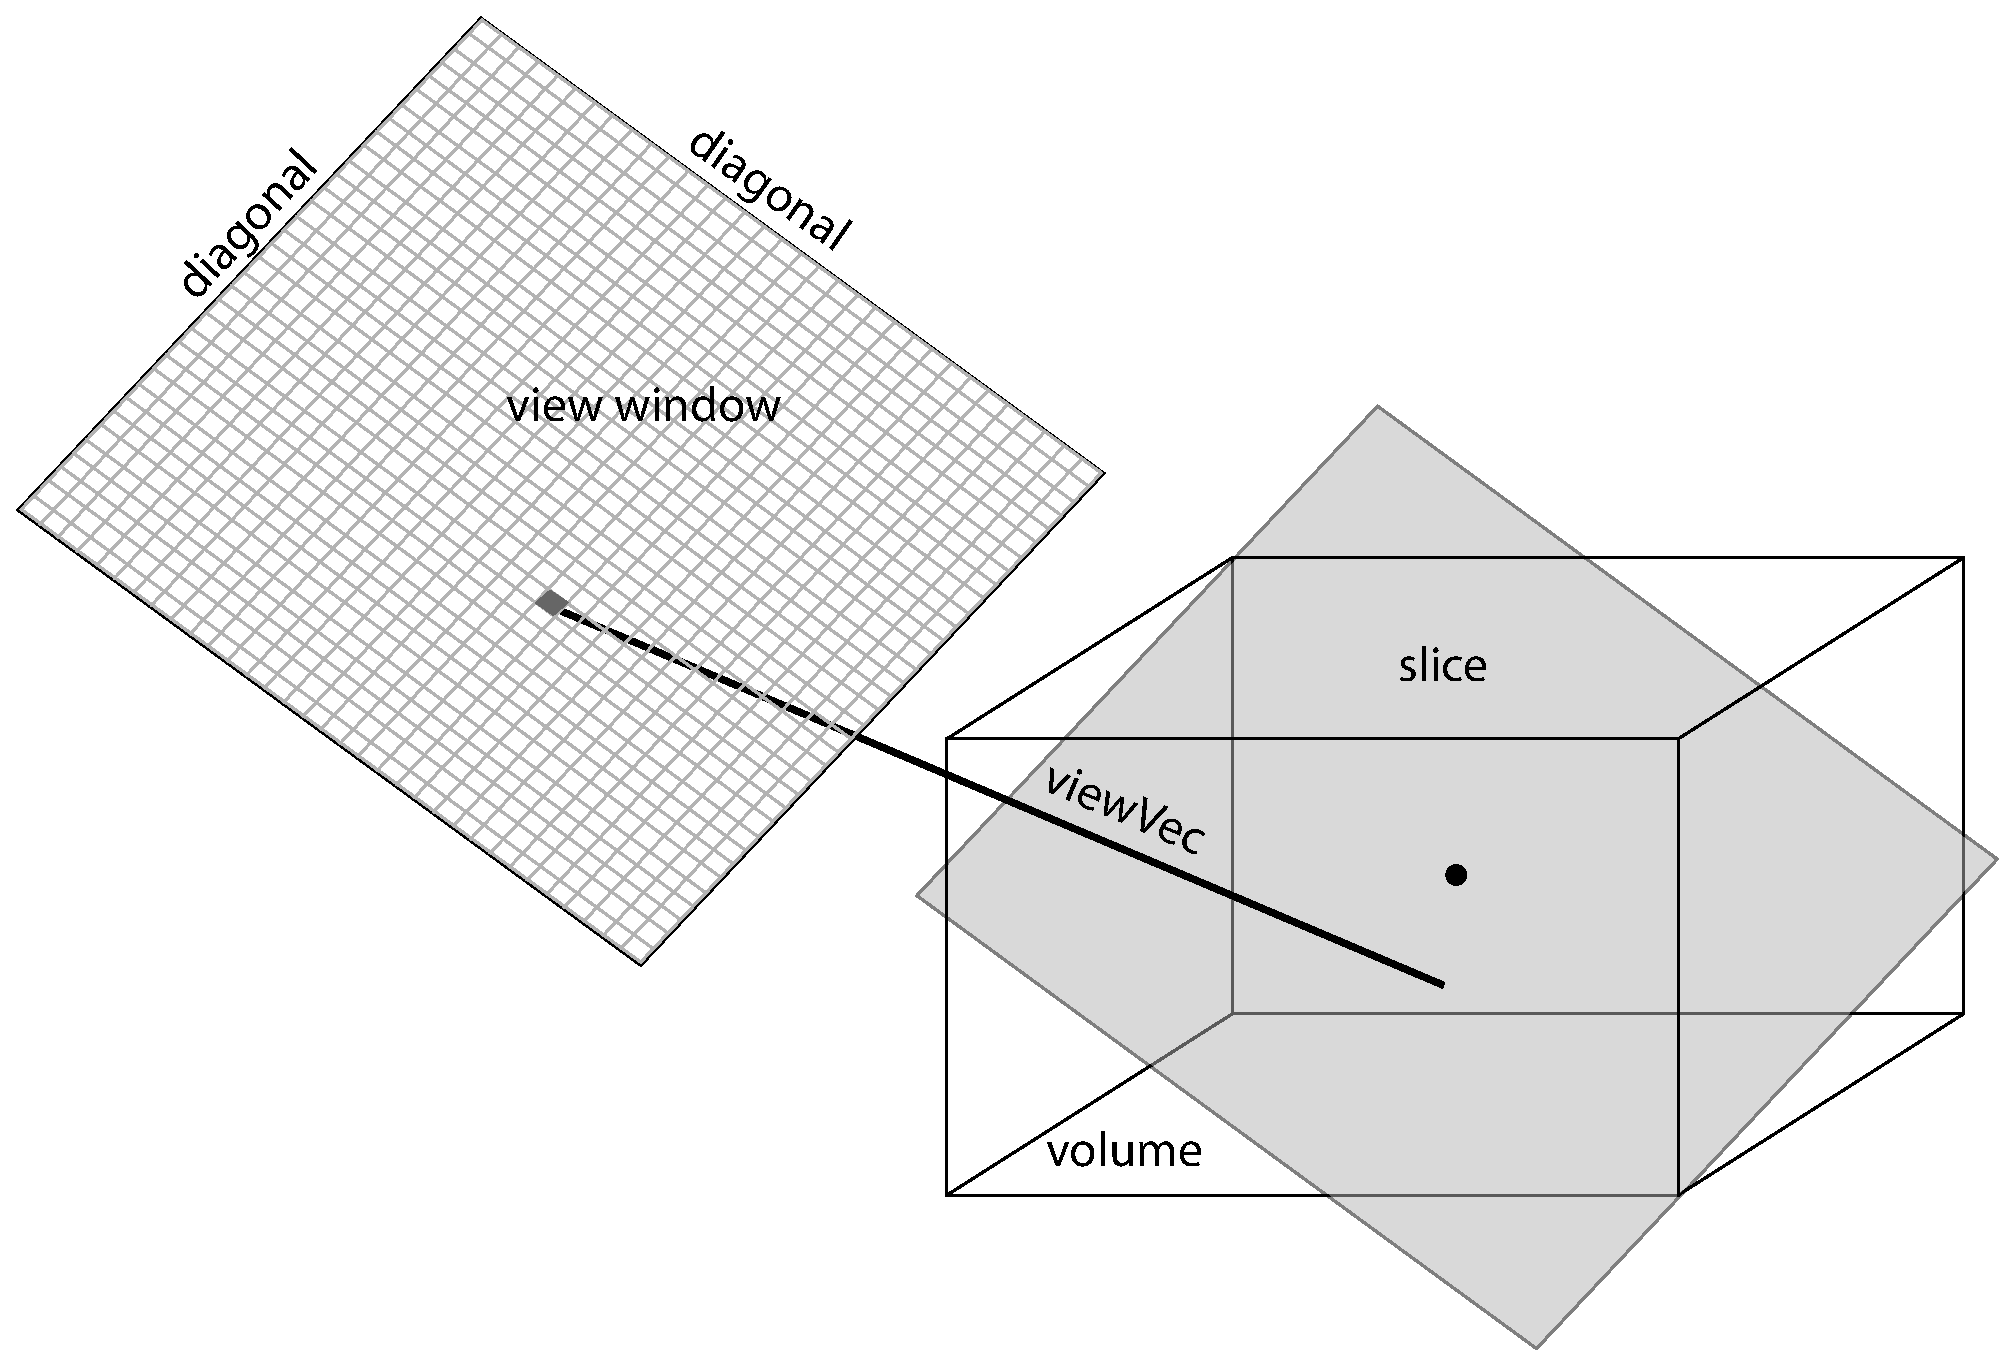
\includegraphics[width=0.8\textwidth]{img/raycaster0.pdf}
    \caption{The initial raycaster application: only a slice of the data within the volume is taken and projected onto the image (screen pixels)}
    \label{fig:raycaster0}
\end{figure}

With this application as a starting point, we devote the upcoming sections to explaining the additional features that were implemented. We start in section \ref{sec:mip} with the implementation of a Maximum Intensity Projection method. We furthermore adjust the interpolation technique for the points on a casted ray from a nearest neighbor interpolation to a tri-linear one. Because the implementation of a MIP greatly reduces the performance of the application, we present several performance enhancement methods in section \ref{subsec:perf_enh}. In section \ref{sec:compositing} we present an alternative implementation for the MIP, namely compositing. Section \ref{sec:opacity} finally describes how ...\todo{!}


\section{Data Set}\label{sec:data}




\section{Tasks}\label{sec:tasks}

In this section we define the visualization tasks that we would like to execute on the given data set. That is, we describe what information we would like to retrieve from the given data. However, before we define these tasks, we provide a framework (i.e., design space) for formulating specific visualization tasks.

\subsection{Framework for Defining Tasks}
In order to formulate a nice and clear visualization task, we define a framework for doing this as presented in \cite{schulz2013design}. Here we distinguish between five different dimensions for each task, namely the \textit{goal} (why is the task pursued?), \textit{means} (how is the task carried out?), \textit{characteristics} (what does the task seek?), \textit{target} (on which part of the data is the task carried out?) and \textit{cardinality} (on how many instances is the task carried out?). We shortly explain these five aspects in some more detail.

For the goal of the task we distinguish between three different types of analyses. We can have an exploratory analysis (or undirected search) that aims at deriving an hypothesis from an unknown data set, a confirmatory analysis (directed search) that aims to verify a found or assumed hypothesis, and finally a presentation that simple exhibits analysis results.

For describing how the task is being carried out we distinguish between three main ways of doing so. These are navigation, (re-)organization and relation. Navigation 'subsumes all means that change the extent or the granularity of the shown data, but that do not reorganize the data itself'. (Re-)organization includes all means that actually adjust the data to be shown by either reducing or enriching it, and relation encompasses all means that put data in context.

Characteristics of the data can be subdivided in low-level data characteristics and high-level ones. Examples of low-level characteristics are data values of a particular data object or the data objects corresponding to a particular data value. Examples of high-level characteristics include more complex data patterns such as trends, outliers, clusters, frequency, distribution, correlation, etc.

The target of the visualization task describes on which part of the data the task is being carried out. This often boils down to a certain (sub)set of the different data attributes.

The cardinality finally specifies which part of the data instances we consider when carrying out the task. For instance just a single one, a certain subset, or just all of them.


\subsection{Chosen Tasks}
With this common framework for formulating visualization tasks defined, we move on to defining the actual tasks we want to perform on our data set about the Dutch municipalities. We mainly distinguish between two different tasks, of which the first one will be divided into two subtasks.

\subsubsection{Task 1}\label{sec:task1}
The first task that we define aims at discovering interesting properties of the given data set, as well as confirming expected properties. This means that this task is actually rather broad, and numerous specific questions can be formulated from it. However, we will define two basic (sub)tasks for analyzing the entire data set, namely\textit{a)'analyze the relations between the different attributes'} in the set, and \textit{b) 'compare the attribute values of the different municipalities with each other'}. The subset of attributes on which we will perform both of these tasks will be the same. This subset will consist of the attributes \texttt{OAD}, \texttt{STED}, \texttt{AANT\_INW}, \texttt{BEV\_DICHTH}, \texttt{AANTAL\_HH}, \texttt{P\_EENP\_HH}, and \texttt{OPP\_TOT}. For convenience we will call this set of attributes $S_{attr}$.

When formally defining task 1a, we observe that we adopt an \textit{exploratory} approach, as we aim at \textit{searching} interesting \textit{relations} between different data set attributes. From this we can (partly) derive the first three dimensions for our 5-tuple task description. The forth dimensions, the target has also been specified already, namely $s_{attr}$. This leaves us with the cardinality. Because we want to discover general relations, we want to look at all data instances (municipalities). However, some relations between attributes may be very obvious. We will therefore also be looking for \textit{confirmation} of these obvious relations, and want to detect possible abnormalities or inconsistencies in them, such as \textit{outliers}. The resulting formal task description then looks like this:

(exploratory|confirmatory, relation-seeking, relations|outliers, $S_{attr}$, all)

For task 1b we can define a somewhat similar task. The main difference is now that we will not be looking at the relations between the different data attributes, but are \textit{comparing} the data values of the different data objects. In this way we again hope to find interesting characteristics such as \textit{outliers} or \textit{clusters}. As with task 1a, we again take $S_{attr}$ as our target and all instances as cardinality.

(exploratory|confirmatory, comparison, outliers|clusters, $S_{attr}$, all)

Specific questions that we could pose for the first of these two subtasks is for instance 'is there a positive relation between the attributes \texttt{AANT\_INW} and \texttt{BEV\_DICHTH}?'. If we think about this for a minute in advance, we may expect that this will indeed be the case. Hence this would be a typical question where we try to confirm our hypothesis, and look for data objects that do not adhere to this. A much more general and exploratory question would be 'which attributes have a typical positive or negative relation with each other?'. Again we may define some expected relations, such as a negative relation between \texttt{OAD} and \texttt{STED}. However, this question really aims for elaborate (though high level) analysis of the data.

For task 1b we can also define a question of which we can already guess the answer. We could for instance confirm that the four largest cities in the Netherlands score the highest on the \texttt{AANT\_INW} attribute. Furthermore we may expect these values to be rather significantly larger than those of the other municipalities. Finally we may again pose a general, exploratory question in the form of 'how are the attribute values of the municipalities distributed for a certain attribute, and can we explain this distribution?'.




\subsubsection{Task 2}\label{sec:task2}
In this task we search for confirmation to a specific question.
This question is formulated based on a hypothesis on which we seek validation.
Once the question is answered it can be used to support the hypotheses.\\
\\
The specific question we want an answer to is whether there are municipalities in the Netherlands that suffer from a high degree of an aging population ('vergrijzing' in Dutch).
This question is based on the hypothesis that the Netherlands is suffering of a high degree aging population.\\
The degree of aging population is based on the inhabitants that are older than 65 years, and the working inhabitants.
The working inhabitants are defined as the age group from 20 till 65, this is not the actual group of working inhabitants but it is a good representation.
\\
The specific question can be described as a formal task description:\\
(\textit{confirmatory, searching localization, attr($P\_00\_14\_JR$, $P\_15\_19\_JR$, $P\_20\_24\_JR$, $P\_25\_44\_JR$, $P\_45\_64\_JR$, $P\_65\_EO\_JR$), all})\\
\\
The formal task describes that the user is searching confirmation among all available 65+-percentage attribute values and the 20- till 64-percentage attribute values, this last attribute is created with a combination of different percentage attributes.
The task is confirmatory, so the user knows what he is looking for and seeking confirmation to what he wants to prove.
The user is looking at low-level data characteristics (localization), this means no complex patterns in the data but simply searching for the high valued attribute values in the data objects (municipalities). 
\section{Techniques}

\subsection{techniques for task 1}
\todo{foreseen pros and cons}

Techniques that can be chosen for this broad exploration of the data include a Parallel Coordinate Plot (PCP) and Scatterplot Matrix (SM). This is because these two techniques enable us to show a lot of different attributes in one large overview. An advantage of the PCP over the SM is however that the PCP tends to take up less space. Also the axes of the SM tend to become very small when numerous attributes are used. This makes it hard to distinguish between single data objects when analyzing the data. When data objects can be be categorized, this problem can be partly overcome by specifying each category with a certain color. However, for our municipalities data set this categorization is not really possible. An imaginable solution for this would be an interactive SM where the user can zoom in on one of the scatterplots. Unfortunately D3 \cite{D3} does not provide such an example, and implementing it ourselves was considered to consume too much time. For these reasons, it was chosen do use a PCP.

con: outliers rack up the scaling -> solution: scale the axes to selection


\subsection{techniques for task 2}
\todo{foreseen pros and cons}

\subsection{techniques for task 3}
\todo{foreseen pros and cons} 
\section{Observations}

\subsection{Observations Task 1}
\todo{what information could be retrieved from the implemented technique?}
\todo{was the task accomplished?}
\todo{pros, cons, improvements}

\begin{figure}[h!]
    \centering
    \includegraphics[width=0.8\textwidth]{img/para_outliers.png}
    \caption{Outliers in the Parallel Coordinate Plot}
    \label{fig:para_outliers}
\end{figure}

\subsection{Observations Task 2}
\todo{what information could be retrieved from the implemented technique?}
\todo{was the task accomplished?}
\todo{pros, cons, improvements}



\bibliographystyle{plain}
\bibliography{bibliography}

\appendix
\section{Appendix: Work breakdown}\label{app:appA}




\end{document}
